\scanpage{37}
\mspage{18}
\uline{Supplement}. Return to a \uline{geometric} proof of \unsure{theorem|Theorem} 2, corollary 1 b). We may assume that $G$ is the generalized Jacobian of $Y$, and it suffices to prove the

\uline{Lemma} \margin{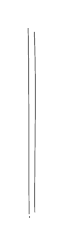
\begin{tikzpicture}[x=0.006cm,y=0.006cm]
\draw[black!55,line width=.35pt] (0,0) .. controls (2,-130) and (1,-266) .. (2,-394);
\draw[black!55,line width=.35pt] (13,-8) .. controls (18,-137) and (13,-266) .. (14,-390);
\fill (3,-400) circle (1.3);
\end{tikzpicture}} Let $Y$ be an anabelian elementary Artin variety, (over $K$ algebraically closed), $Y\hookrightarrow J_Y^1$ its embedding in its generalized Jacobian, $u\in J_Y^0(k)$ and $U$ a nonempty open subset of $Y$, such that $U+u\subset Y$. Then $u=1$\inserted{, or again: the map $x\mapsto xu$ from $U$ to $Y$ is the identity.}

By dévissage, we are reduced to the case where $Y$ is a curve. First suppose it complete, so that $U+u\subset Y$ implies $Y+u\subset Y$ -- then the result is well known This follows for example from the formula for fixed poin\textsuperscript{ts}, which implies that $\tau_u\mid Y$, \inserted{if it is not the identity,} has $2-2g$ fixed poin\textsuperscript{ts}, which (since $g\geq2$ because of the anabelian hypothesis) is absurd.

This therefore \deleted{\unsure{means}} \inserted{implies}, in the general case, \inserted{at least if $g\neq1$,} that the image of $u$ in the abelian part of $J_Y^0(k)$ is zero.

\margin{If $g\geq2$, replacing $Y$ by $\widehat Y$ if necessary, we may assume $Y$ complete. If $g=1$ or 0, cf homological argument below}
\margin{serves no purpose here}

\deleted{[[Now according to the known structure of $J_Y^0$ as an extension of $J_{\widehat Y}^0$ by a torus $\mathbb G_m^I/\mathbb G_m$ (where $I=\widehat Y\unsure{\setminus|-}Y$) $u$ is identified with an element of $(\mathbb G_m^I/\mathbb G_m)_{\unsure{0}}(k)$, thus is defined by $(\lambda_i)_{i\in I}$, the $\lambda_i\in k^*$, which serve to construct a line bundle}
\margin{36}
